\documentclass[10pt,a4paper]{article}
\usepackage[utf8]{inputenc}
\usepackage[english]{babel}
\usepackage{amsmath}
\newcommand*{\boxcolor}{mypink1}
\makeatletter
\renewcommand{\boxed}[1]{\textcolor{\boxcolor}{%
\tikz[baseline={([yshift=-1ex]current bounding box.center)}] \node [rectangle, minimum width=1ex,rounded corners,draw] {\normalcolor\m@th$\displaystyle#1$};}}
\makeatother
\usepackage[dvipsnames]{xcolor}
\definecolor{mypink1}{cmyk}{0, 0.7808, 0.4429, 0.9}
\usepackage{mathrsfs}
\usepackage{amsfonts}
\usepackage{amssymb}
\usepackage{tikz}
\usepackage{cancel}
\usetikzlibrary{shapes.geometric}
\newcommand{\warningsign}{\tikz[baseline=-.75ex] \node[shape=regular polygon, regular polygon sides=3, inner sep=0pt, draw, thick] {\textbf{!}};}
\usepackage{tcolorbox}
\usepackage{graphicx}
\usepackage{commath}
\usepackage{esint}
\usepackage[left=2cm,right=2cm,top=2cm,bottom=2cm]{geometry}
\usepackage{tikz}
\usetikzlibrary{calc}
\usepackage{bm}
\usepackage{xcolor}
\usepackage{soul}
\newcommand{\mathcolorbox}[2]{\colorbox{#1}{$\displaystyle #2$}}
\newcommand{\hlfancy}[2]{\sethlcolor{#1}\hl{#2}}

\newcommand{\prob}{\mathcal{P}}

\newcommand{\particle}[4]{\draw (#1, #2) circle (3pt);
    \draw[thick, ->] (#1, #2) -- (#1 + #3, #2 + #4);}

\author{Marco Biroli}
\title{ODG Final}
\begin{document}
\maketitle

\section{At which speed does one have to move to stay in the zone of total eclipse of the sun?}
When a total eclipse was visible in Paris at 10 it's counter part is visible in New York around 14h30 this means that to follow the eclipse one would have had to travel approximatly $5\cdot 10^{3}$ kilometers in 4h30min. Which gives an approximate speed of $5\cdot{10^3}/5 = 10^3 \text{km}.\text{h}^{-1}$.


\section{Estimate the time needed for the diffusion of a water molecule from one side to the other of an Olympic pool.}
From the course and a simple dimensional analysis we know that:
\[
R \sim \sqrt{D t} \Rightarrow t \sim R^2 D^{-1}
\]
Where $R$ will be the length of the pool $\sim 50 \,m$ and $D$ the diffusion coefficient of water. From the course (Lecture 1) we also know that typical magnitude of diffusion coefficient with water is around $10^{-5} \text{   cm}^2.\text{s}^{-1}$. Hence we get:
\[
t \sim 2 \cdot 10^7 \cdot 10^5 = 2 \cdot 10^{12} \text{ s}
\]


\section{How much data is transfered in the world every second?}
We start by trying to estimate what is the average internet consumption per person. We assume that internet traffic will be majorly dominated from video streaming and messaging. Other activities like emails, downloads, google searches and so on either are less frequent or of a much smaller size. Then assuming on average from streaming people stream videos at $1920\times 1080$ pixels quality each pixel being encoded on 1 byte this gives an approximate $2\cdot 10^6$ bytes per image. A video consists usually of $30$ to $60$ images per second and hence a video will cost approximately $10^8$ bytes per second. Messaging is much less costly however much more frequent hence one could think of taking it into account. One message would have an approximate size of $10^2$ bytes. Now a given person will probably spend on the order of a few hours streaming and send an average of $10^2$ messages per day (since email/text-messages/google searches have more or less the same size we can count them all together here). Which means that per day a person would consume something of the order of $3 \cdot 10^3 \cdot 10^8 + 10^2 \cdot 10^2$ now as we initially predicted notice that streaming is hugely dominant in terms of traffic. Now averaging over a day gives an average traffic of $3 \cdot 10^{-5} \cdot 10^4 \cdot 10^8 = 3 \cdot 10^7$ bytes per second per person. Now we assume that around half of the earth uses internet at any given second (discrepancies w.r.t. poverty are probably more or less equally accounted for by richer people owning more than one electronic device) so we get a total traffic of $10^9 \cdot 3 \cdot 10^7 = 3 \cdot 10^{16}$ bytes per second. Now taking into account that applications use compression methods to reduce traffic, we estimate the average efficiency of these compression methods to around $30\%$ the total traffic is brought down to:
\[
10^6 \text{Gb}.\text{s}^{-1}
\]
Which when compared to real life data is very close to the actual result: $94\,201 \text{Gb}.\text{s}^{-1}$\\
https://www.internetlivestats.com/one-second/\#traffic-band

\section{Create an experiment to measure the temperature with a laser of a gas with two very close excited states.}
\subsection{Problem Proposed}

In this problem we are going to consider a simplified model where we will analyze alkali atoms (rubidium (because that is the only one for which I could find data on the internet)) which have a mass of $84$ atomic mass units (m = $84 \cdot 1,660539040(20) \cdot 10^{-27}$ kg) with three energy levels: the ground state (0), an excited state corresponding to a transition at 780 nm (1) and a second state approximately $2\pi \cdot 1$ GHz above the first one (2). The energy being defined as $E = \frac{hc}{\lambda}$, we know that the gap between the (0) and (1) [$E_{0\rightarrow 1} \approx 2,55\cdot 10^{-19}$ J] will be big compared to the gap between (1) and (2) [$E_{1\rightarrow 2} \approx 6,62\cdot 10^{-25}$ J]. The energy states of the alkali atom are thus as follow,

\begin{figure}[h!]
    \centering
    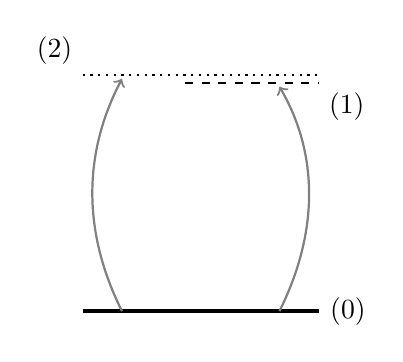
\begin{tikzpicture}
    \draw[thick, dotted] (0, 0) node[above left] {(2)} -- (3, 0);
    \draw[thick, dashed] (1.3, -0.1) -- (3, -0.1) node[below right] {(1)};
    \draw[ultra thick] (0, -3) -- (3, -3) node[right] {(0)}; 
    \draw[thick, ->, gray] (0.5, -3) .. controls (0, -2) and (0, -1) .. (0.5, -0.05);
    \draw[thick, ->, gray] (2.5, -3) .. controls (3, -2) and (3, -1) .. (2.5, -0.15);
    \end{tikzpicture}
    \caption{Sketch of the energy states of the alkali atom}
\end{figure}

We assume that the states (1) and (2) have the same bandwidth of $2\pi \cdot 30$ MHz. We neglect the transitions that could occur between states (1) and (2) and assume interactions solely between (0) and (1) and (0) and (2). \\ \\
We then design the following protocol:
\begin{enumerate}
\item Fill a transparent (for the wavelengths considered) glass cell with the gas in consideration.
\item Saturate the gas (pump half of the atoms in their excited states and half in the ground states).
\item Send lasers of varying wavelengths through the sample retro-reflect it and measure the intensity with a photo-diode as show in Figure \ref{2} below.
\end{enumerate}

\begin{figure}[h!]
    \centering
    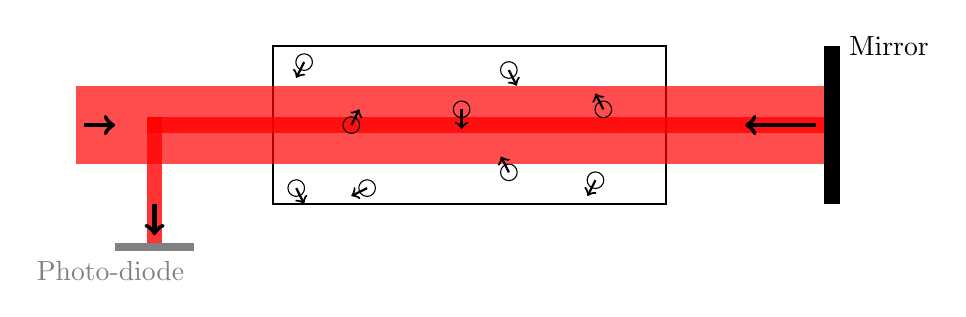
\begin{tikzpicture}
    \draw[thick] (0, 0) rectangle (5, 2);
    \fill (7, 0) rectangle (7.2, 2) node[right] {Mirror};
    \fill[gray] (-2, -0.5) rectangle (-1, -0.6) node[below left] {Photo-diode};
    \fill[red, opacity=0.7] (-2.5, 0.5) rectangle (7, 1.5);
    \draw[ultra thick, ->] (-2.4, 1) -- (-2, 1);
    \fill[red, opacity=0.8] (-1.6, 0.9) rectangle (7, 1.1);
    \draw[ultra thick, ->] (6.9, 1) -- (6, 1);
    \fill[red, opacity=0.8] (-1.6, 1.1) rectangle (-1.4, -0.5);
    \draw[ultra thick, ->] (-1.5, 0) -- (-1.5, -0.4);
    \draw (3, 1.7) circle (3pt);
    \draw[thick, ->] (3, 1.7) -- (3 + 0.1, 1.7 - 0.2);
    \draw (1.2, 0.2) circle (3pt);
    \draw[thick, ->] (1.2, 0.2) -- (1.2 - 0.2, 0.2 - 0.1);
    \draw (4.2, 1.2) circle (3pt);
    \draw[thick, ->] (4.2, 1.2) -- (4.2 - 0.1, 1.2 + 0.2);
    \particle{0.3}{0.2}{0.1}{-0.2}
    \particle{0.4}{1.8}{-0.1}{-0.2}
    \particle{4.1}{0.3}{-0.1}{-0.2}
    \particle{2.4}{1.2}{0}{-0.25}
    \particle{3}{0.4}{-0.1}{0.2}
    \particle{1}{1}{0.1}{0.2}
    \end{tikzpicture}
    \caption{Experimental set up}
    \label{2}
\end{figure}
The intensity graph we expect to obtain after these measurements is shown in Figure \ref{3}. Using these informations we will try to answer the question, 
\begin{center}
    \textbf{What is the temperature of the alkali atoms?}
\end{center}
\begin{figure}[h!]
    \centering
    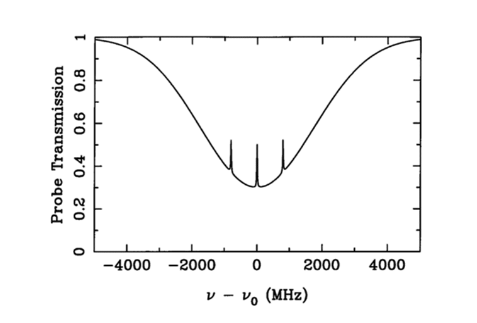
\includegraphics[width = 0.7\textwidth]{intensityGraph}
    \caption{Intensity graph after analysis of the retro-reflected beam taken from [1].}
    \label{3}
\end{figure}


\section{Explain the phenomena behind the intensity graph}
\begin{figure}[h!]
    \centering
    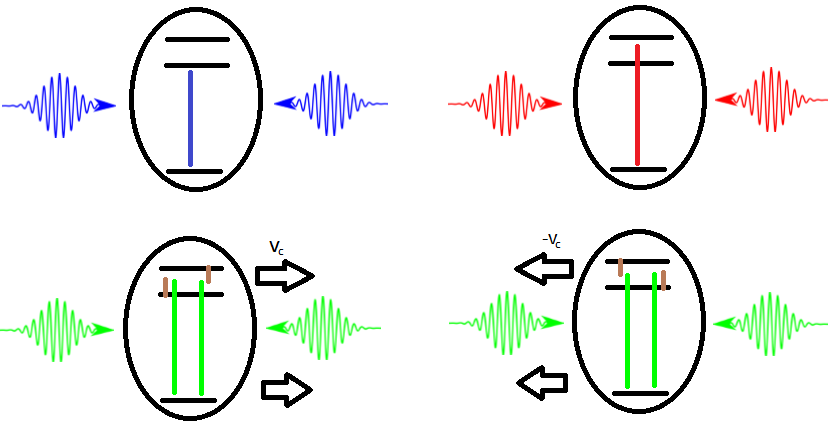
\includegraphics[width = \textwidth]{DopplerTransitions.png}
    \caption{Schema of possible double transitions explaining peak 1 (blue), 2 (green) and 3 (red).}
\end{figure}
On the intensity graph we can isolate three sharp peaks around the minimum of the graph. To what do these 3 peaks correspond and to what corresponds the general form of the graph? \\ \\ The general form of the graph is a consequence of the Doppler shift. Atoms in the cavity move at various velocities, hence will perceive the frequency of the light according to the Doppler shift formula $\omega_{perceived} = \omega _{lab frame} (1-v/c)$. Thus, atoms can absorb and emit on a wide range of frequencies, explaining the general trend of the curve. \\ \\
Let us explain the three sharp peaks observed. The left most sharp peak corresponds to transitions between the ground state (0) and the first excited state (1) when the alkali atoms are relatively still with respect to the direction of movement of the laser. The right most peak corresponds transitions between the second excited state (2) and the ground state (0) when the alkali atoms are relatively still in the direction of movement of the laser. The middle sharp peak is explained by the Doppler shift, that we see hereafter. \\ \\
Observe Figure 4. The two transitions that are the simplest to understand are the blue and red transitions. When a photon carrying just the right amount of energy to excite an electron from the ground state to the first or second excited state meets an atom that is standing still, then the photon will excite  and successively de-excite by stimulated emission the atom on the way back. The stimulated emission will multiply the amount of photons coming back which explains why we observe a peak in the absorption graph. (Corresponding to the left-most and right-most peaks). The third transition (in green) is a bit harder to understand. Since the gas is at a non-zero temperature the atoms will be undergoing some motion. If a photon having the exact average of the energies required for the first and second transitions meets an atom that is traveling at a very specific speed $v_c$ (that we will compute later), then the Doppler shift will make it so that the atom perceives the photon as having the right amount of energy for a transition with the first (resp. second) on the way in and second (resp. first) on the way back. This explains the middle peak. \\\\
Notice that the spacing between the peaks is equal. Indeed, denote by $\omega_m$ the frequency corresponding to the middle peak. It must satisfy:
\begin{align*}
    \begin{cases}
    \omega_0 = \omega_m (1-v/c) \\
    \omega_1 = \omega_m (1+v/c) \\
    \end{cases}
    \implies \omega_0 + \omega_1 = 2\omega_m \iff \omega_m = \frac{\omega_0 + \omega_1}{2}
\end{align*}

To resume: The left most peak corresponds to transitions from (0) and (1) and the right most peak to transitions from (0) and (2) when the alkali atoms are relatively still with respect to the direction of movement of the laser. The middle peak is a combination of the two transitions explained by the Doppler shift that is implied by the moving atoms. 

\begin{comment}
Therefore our final figure is the superposition of the two Gaussians corresponding to the here above mentioned mechanisms, and we get the sketch of Figure 5.


\section{Finding the temperature with the superposition of the Gaussians}

\begin{figure}[h!]
    \centering
    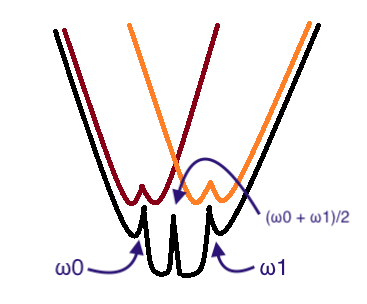
\includegraphics{Superposition.PNG}
    \caption{Superposition}
\end{figure}

We have two Lorentzian profiles, the first one corresponding to the transition from ground level to the first energy level, and the second one corresponding to the transition from ground level to second level. The intensity graph is hence a superposition of these two functions, as we can see from  Figure 5. As it has already been explained, there are three situations where we can have that an atom first absorbs and then emits by stimulation, and we can infer them from Figure 5. Indeed we see that there are three small peaks, and we can identify that the left one corresponds to sending a laser with frequency $\omega_0$ (corresponding to the frequency necessary to reach the first energy level from the ground state), the middle one is the case where absorption occurs in one energy level and stimulated emission in the other, thanks to the Doppler shift analyzed before, this frequency is $\frac{\omega_0+\omega_1}{2}$. The rightmost one corresponds to the transition to the second energy level, with frequency $\omega_1$ (frequency to reach the second  energy level from the ground state).
By simplicity, since we don't have an explicit expression for the Lorentzian profile, we will consider the superposition of the related Gaussians. The first Gaussian is centerd at $\omega_0$, and the second one at $\omega_1$. Moreover, being their sum a symmetrical function with respect to the central peak ($\frac{\omega_0+\omega_1}{2}$), these Gaussians have the same extrinsic broadening (i.e. the same full width at half maximum), which we call $\Delta \omega$. It is the quantity we are interested in as we can relate it directly to the temperature of the atoms in our system. Now we call $f$ the superposition of the two Gaussians, we get
$$f(x)=e^{-\frac{(\omega-\omega_0)^2}{2\Delta\omega^2}}+e^{-\frac{(\omega-\omega_1)^2}{2\Delta\omega^2}}$$
Now if we call $\delta\omega=\omega_0-\omega_1$ we get:
$$\frac{f(\omega_0)}{f(\frac{\omega_0+\omega_1}{2})}=\frac{1+e^{-\frac{-\delta\omega^2}{2\Delta\omega^2}}}{2e^{-\frac{\delta\omega^2}{8\Delta\omega^2}}}.$$

We know the value of $r:=\frac{f(\omega_0)}{f(\frac{\omega_0+\omega_1}{2})}$ since we can find it from the graph. The graph has no scale but this is not an issue as we want a quotient between two quantities. 
Then we call $x:=e^{-\frac{\delta\omega^2}{8\Delta\omega^2}}$, and we obtain 
$$r=\frac{1+x^4}{2x}\Leftrightarrow x^4-2rx+1=0$$
Now from the graph, by measuring with the ruler the ratio between $f(\omega_0)$ and $f(\frac{\omega_0+\omega_1}{2})$, we find that $r=0.94$ (we need to take the modulus of $r$ since actually in the graph the gaussians are reversed wrt the frequency axis) and thanks to Wolfram Alpha we find the solution $x=0.6$.
Then we know the value $\delta\omega=\omega_0-\omega_1=10^9GHz$ from which we obtain
$$\Delta\omega^2=-\frac{\delta\omega^2}{8\ln(x)}= 25\cdot10^{16} Hz$$


Then from $\Delta\omega=\sqrt{\frac{k_BT\omega_0^2}{mc^2}}$
and using $m$ as reported at the beginning of the pdf, we get
$$T=\frac{\Delta\omega^2mc^2}{k_B\omega_0^2}=\frac{25\cdot 10^{16} \cdot 40\cdot 1.66\cdot 10^{27}\cdot 9\cdot10^{16}}{3.8^2\cdot 10^{28}\cdot 1.38\cdot 10^{-23}}=750 K$$

\end{comment}

\section{Finding the temperature using Maxwell-Boltzmann distribution.}
\subsection{Preliminary work.}
It might not be obvious how we can can link the ratio in peak intensities with the Maxwell-Boltzmann distribution, we will try to explain it here. We saw initially that the peaks are due to the stimulated emission of particular photon-atom interactions. These peaks are not infinitly thin because the transitions have an intrinsic bandwidth w.r.t. the atom, but here we are only concerned with the maxima of the peaks so we will not pay much attention to the rest. Every double transition creates one re-emmitted photon and the number of re-emmitted photons is proportional to the "extra" received intensity which gives the three peaks we observe. This chain of proportionality re-written in probability translates to:
\[
\prob(\text{transition}) \propto \Delta I(\text{transition})
\]
For a transition to occur we need three things, the right photon, the right atom and for the transition to actually occur. Now given the right photon and atom we assume that the probability of the transition actually occurring is a constant. We also assume that the distribution of frequencies in the incoming photons is uniform (i.e. all the lasers we are using have the same properties such as intensity), so the probability of finding the right photon is also a constant. Then we see that the only varying factor is the probability of finding the right atom. For transitions 1 and 3 this corresponds to finding an atom that has speed $v_x = 0$, where we take $x$ to be the axis along the propagation of the beam in the gas. For transition 2 it corresponds to finding an atom with speed $v_x = \pm v_c$. It follows that:
\[
\begin{cases}
\prob(v_x = 0) \propto \Delta I_{13}\\
\prob(v_x = v_c) + \prob(v_x = -v_c) \propto \Delta I_2
\end{cases}
\Rightarrow \frac{\prob(v_x = v_c) + \prob(v_x = -v_c)}{\prob(v_x = 0)} = \frac{\Delta I_2}{\Delta I_{13}}
\]
Then assuming that the distribution of the gas follows a Maxwell-Boltzmann distribution ($F$) then we get that:
\begin{equation}
    \frac{2F(v_c)}{F(0)} = \frac{\Delta I_2}{\Delta I_{13}} = r
\end{equation}

\subsection{Finding $v_c$.}
We know that $v_c$ has to solve the following equation:
\[
\omega_0 = \frac{\omega_0 + \omega_1}{2} \left( 1 - \frac{v}{c}\right) \Leftrightarrow v_c = c\left( 1 - 2\frac{\omega_0}{\omega_0 + \omega_1}\right) = 385 \text{ m.s}^{-1}
\]

\subsection{Conclusion.}
We know that the Boltzmann distribution is given by:
\[
F(v_x) \propto \exp\left( -\frac{v_x^2 m}{2k_B T} \right)
\]
Then we get that:
\[
2\frac{F(v_c)}{F(0)} = 2\exp\left( -\frac{v_c^2 m}{2 k_B T} \right) = r
\]
Solving for $T$ we get that:
\[
T = \frac{v_c^2 m}{2 k_B \ln\left(\frac{2}{r}\right)}
\]
Now from the graph found in [1] and measuring the peaks by hand from the image, we get that $r \approx \frac{5}{4}$ which gives:
\[
T = 740 \text{ K}
\]
The papers never mention the temperature at which the potassium gas is. However from the internet we can see that the typical temperature of potassium cells are around $300-1000$ K [2]. So we get the good order of magnitude.

\section{References}
\begin{enumerate}
\item[[1]] http://pmaweb.caltech.edu/~ph77/labs/optics/satabs1.pdf
\item[[2]] https://www.thorlabs.com/newgrouppage9.cfm?objectgroup\_id=1470
\end{enumerate}

\end{document}